% \subsection{Peak values of the streamwise spectra}

\begin{figure}
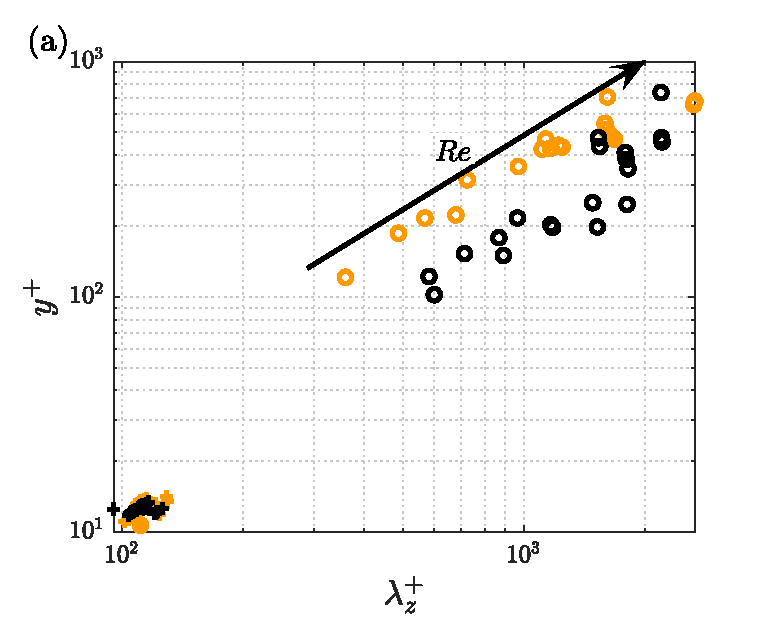
\includegraphics[width=0.49 \textwidth]{peak_uu_ltau_ltau.eps}
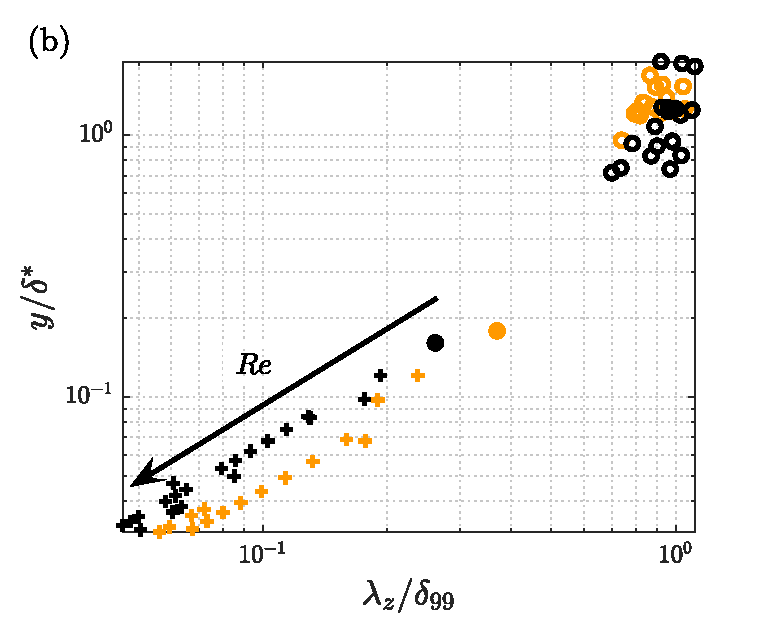
\includegraphics[width=0.49 \textwidth]{peak_uu_dstar_d99.eps}
\caption{ \label{fig:peaks} Representation of the peaks in the premultiplied streamwise power-spectral density $k_z\phi_{uu}$ in (a) inner scaling and (b) scaling with boundary-layer and displacement thicknesses. Crosses denote the inner peak (IP) and circles for the outer peak (OP). Note that in (a) the inner peaks collapse by scaling the wall-normal position $y$ and the wavelength $\lambda_z$ in viscous units, and in (b) the outer peaks collapse when scaling $y$ and $\lambda_z$ with $\delta^*$ and $\delta_{99}$, respectively. The black arrows show the direction of increasing Reynolds number.}
\end{figure}

The near-wall peak of $\overline{u^2}$ is closely connected with the spectral near-wall peak of $k_z\phi_{uu}$, thus it is natural to use the viscous scaling for this region as shown in Fig.~\ref{fig:peaks}(a) for a number of profiles between $Re_{\tau}=1000$ and 2000. This figure shows that the spectral inner peaks are located at approximately the same location for both APG and ZPG, at $y_{s \rm IP}^+\simeq 12.5$, without a clear trend due to the resolution taken for the spectra close to the wall.
The spanwise wavelenghts of the near-wall peak also collapse using inner scaling to a value $\lambda_{z,s \rm IP}^+ \approx 112$.

The outer peak of the RS is related with the spectral outer peak, and Fig.~\ref{fig:peaks}(b) shows that this spectral peak collapses in the premultiplied spectra. In particular, the wall-normal location of the outer peak scales with $\delta^*$ as in Ref.~\cite{Kitsios2017}, while the spanwise wavelength $\lambda_z$ scales with $\delta_{99}$ \cite{Lee2017, bobke2017}. Again, due to the resolution of the spectral data, the values are slightly scattered. 
Our results show that the average $y_{s \rm OP}/\delta^*$ is 1.3 for the APG and 1.1 for the ZPG. The average spanwise wavelenghts $\lambda_{z, s \rm OP}/\delta_{99}$ are 0.91 for the APG and 0.96 for the ZPG.
Considering the collapse of the inner and outer peaks in their respective scalings, then $y^+_{s \rm IP}/\lambda^+_{z, s \rm IP}=C_1$ and ($y_{s \rm OP}/\delta^*)/(\lambda_{z, s \rm OP}/\delta_{99}) = C_2$ are constant values. With the values above we obtain $C_1 \approx 0.1$ (for both ZPG and APG), and $C_2 \approx$ 1.43 for APG and 1.15 for ZPG.
Then the curves that the spectral outer peaks follow in Fig.~\ref{fig:peaks}(a) follow Eq.~(\ref{eq:curve_sOP}), and the spectral inner peaks in Fig.~\ref{fig:peaks}(b) follow Eq.~(\ref{eq:curve_sIP}). Note that $f(Re, \rm PG) = \delta^*/\delta_{99}$, where ${\rm PG}$ denotes the pressure-gradient magnitude. 
\begin{equation}
    y_{s \rm OP}^+ = \frac{y_{s \rm OP}/\delta^*}{\lambda_{z, s \rm OP}/\delta_{99}} \frac{\delta^*}{\delta_{99}} \lambda_{z, s \rm OP}^+  = C_2 f(Re, \rm PG) \lambda_{z, s \rm OP}^+
    \label{eq:curve_sOP}
\end{equation}
\begin{equation}
        \frac{y_{s \rm IP}}{\delta^*} = \frac{y_{s \rm IP}^+}{\lambda^+_{z, s \rm IP}} \frac{\delta_{99}}{\delta^*} \frac{\lambda_{z, s \rm IP}}{\delta_{99}}  = C_1 \frac{1}{f(Re, \rm PG)} \frac{\lambda_{z, s \rm IP}}{\delta_{99}}.
        \label{eq:curve_sIP}
\end{equation}

Since $\delta^*$ and $\delta_{99}$ are outer scales that can be measured in experiments~\cite{diagnostic_Vinuesa}, Eqs.~(\ref{eq:curve_sOP}) and (\ref{eq:curve_sIP}) can be useful to estimate the location of the inner and outer spectral peaks in experiments where the spectra cannot be easily measured. Also note that our results for $y_{\rm OP}$ reported in Pozuelo {\it et al.}~\cite{Pozuelo_JFM_22} are in agreement with Refs.~\cite{Kitsios2017, Maciel_2018, Sanmiguel_PRF}, while $y_{s \rm OP}$ also scales with $\delta^*$ as in Kitsios {\it et al.}~\cite{Kitsios2017}, in a case where the APG is at the verge of separation. The difficulties to distinguish trends using $\delta^*$ or $\delta_{99}$ arise from the fact that we have a mild APG, where $\delta^*/\delta_{99}$ decreases very slowly with Reynolds number.
For larger APG magnitudes, the decay of $\delta^*/\delta_{99}$ is larger with Reynolds number, as can be observed when comparing the results for an APG at the verge of separation shown in Ref.~\cite{Kitsios2017} and the mild-APG in this work. The values for $y_{s \rm OP}/\delta^*$ are similar in both studies, confirming the $\delta^*$ scaling.
As for the wavelength $\lambda_{z,s \rm OP}$, the scaling with $\delta_{99}$ leads to similar trends for the ZPG and the APG simulations as those documented in Refs.~\cite{Lee2017, bobke2017}.

The magnitudes of the peaks are also relevant, since they indicate the energy scale that can be used to scale the energy contours of different regions.
Pozuelo~{\it et~al.}~\cite{Pozuelo_JFM_22} reported that $\overline{u^2}^+_{\rm IP}$ grows with Reynolds number and APG, however, we have observed that the values of the spectral near-wall peak appear to be constant with the Reynolds number and the value for the ZPG case is slightly higher ($\overline{u^2}^+_{s \rm IP}=3.6$) than that of the APG case ($\overline{u^2}^+_{s \rm IP}=3.4$).

Although the ZPG data does not exhibit an outer peak in the RS, the outer region scales with the edge scaling as well as the APG \cite{Pozuelo_JFM_22}; here we assess whether the spectral outer-peak magnitude scales using the square of the edge velocity $U_{e}^2$, 
which is determined in APG TBLs following the methodology described in Ref.~\cite{diagnostic_Vinuesa}.
Our results show that the variation of the values obtained in the outer peak of $k_z\phi_{uu}/U_e^2$ was too large to determine any trend, however, the average level is higher for the APG ($\simeq 4.5 \times 10^{-3}$) than for the ZPG case ($\simeq 3.4 \times 10^{-3}$).
